
\chapter{Tracking und Gestenerkennung}

\section{Aufgabenstellung}
\label{kinect_aufgabenstellung_sec}
\todo[inline]{Author hinzufügen}
\authorsection{Kinect-Gruppe}

Die Kinect-Gruppe bekam die Aufgabe, durch Verarbeitung eines Video- und
 Tiefenbildes eine Person zu verfolgen und ihre speziellen
 Körperhaltungen/Gesten/Bewegungen als Kommandos zu interpretieren.
 Um die Bedürfnisse der anderen Gruppen zu erfüllen, mussten wir den Geschwindigkeitsvektor des verfolgten Menschen und die
 erkannte Geste als Ausgabewerte unseres Moduls weitergeben. Der Videostrom wurde von einem Kinect-Sensor akquiriert.
\vspace{0.3cm}

\noindent Output-Daten mit Nummerierung (\lstinline{openni_source_test SO}):
\begin{enumerate}[start=0]
  \item X-Position des Benutzers
  \item Y-Position des Benutzers
  \item Betrag der Benutzers Geschwindigkeit
  \item Richtung der Benutzers Geschwindigkeit
  \item X-Komponente des Geschwindigkeitsvektors
  \item Y-Komponente des Geschwindigkeitsvektors
  \item Erkannte Geste
  \item Benutzer anwesend
\end{enumerate}

\section{Grundlagen Kinect}
\label{kinect_grundlagen_sec}
\todo[inline]{Author hinzufügen}
\authorsection{Kinect-Gruppe}

Sowohl die Bildqualität von Sensoren, als auch die Verarbeitungsalgorithmen zeigten eine erhebliche Entwicklung in den letzten Jahren.
 Heutzutage sind 3D-Entfernungskameras durch rapide Entwicklung des
 Entfernungsbildaufnahmeverfahren für breite Anwenderkreise erschwinglich
 (unter anderem Microsoft Kinect oder Asus Xtion PRO LIVE).
 Darum können neben 2D Farbbildern immer häufiger 3D-Bilder in Anspruch genommen
 werden. Bewährte Tatsache ist, dass Tiefenkarten eine viel robustere Darstellung geben, als herkömmliche Intensitätsbilder.
 
Im \gls{fzi}-Labor steht eine Kinect Kamera für die Datenakquirierung zur
 Verfügung, die ursprünglich als Zubehör der Microsoft XBOX 360 Spielkonsole
 entwickelt wurde. Der größte Vorteil dieses Sensors liegt in seinem Preis. Eine
 solche Kamera ist bereits für ca 100 Euro erhältlich und wird aufgrund dessen
 immer öfter verwendet.
 
Da die Kinect gleichzeitig sowohl 2D Farbbilder als auch 2.5D Entfernungsbilder liefert, gibt es die Möglichkeit, Verarbeitungsmethoden beliebig zu vermischen.
 Obwohl vielversprechend beschränkten wir uns, wegen hohen Rechenaufwandes, auf
 die Verarbeitung von 2.5D Bildern.
\vspace{0.3cm}

\subsection{Technische Daten}
\label{kinect_umsetzung_technische_daten}
\authorsection{\editorhamza}

\subsubsection{Tiefensensor}
\label{kinect_umsetzung_tiefensensor}

Dieser Sensor besteht aus der Kombination einer 830nm Laser Diode und einem Tiefensensor \gls{cmos} welcher die reflektierten Infrarotstrahlenempfangen kann. Aus der Laufzeit kann so die Tiefe der einzelnen Punkte berechnet werden.

\begin{itemize}
	\item Auflösung: 640x480 Pixels
	\item Tiefenbereich: 0.5m - 10m, Ideal 2m-2.5m
	\item Tiefengenauigkeit: 1cm
\end{itemize}

Ein Tiefenbild besteht somit aus 640x480 Pixeln mit je einer Tiefeninformation proPixel. Diese Tiefeninformation bewegt sich in einem Bereich von 50cm bis 1000cm mit einer Auflösung von 1cm. Pro Sekunde liefert der Kinect-Sensor 30 Tiefenbilder.

\subsubsection{Kamerasensor}

Neben dem Tiefensensor besitzt die Kinect eine normale \gls{rgb}-Kamera. Diese löst mit 640x480 Pixeln auf.

\subsubsection{Audio}

Der Kinect-Sensor ist mit 4 Mikrofonen ausgestattet. Mit diesen ist eine 3D Lokalisierungmöglich. Der Zugriff auf die Audio-Daten ist jedoch noch mit keinem Framework möglich und es sind auch keine weiteren Informationen bekannt.

\subsubsection{Neigesteuerung}

Der Kinect-Sensor beinhaltet einen 3D-Neigesensor und einen Motor mit welchem der Neigungswinkel gegen vorne angepasst werden kann. Der Neigungswinkel beträgt zwischen $-31^\circ$und $+30^\circ$ relativ zum Standfuss.

\subsubsection{LED-Steuerung}

Das Integrierte \gls{led} kann ebenfalls angesteuert werden. Folgende Modus sind möglich:

\begin{itemize}
	\item \gls{led}-Ausgeschaltet
	\item Grün
	\item Rot
	\item Gelb (Orange)
	\item Gelb (Orange) blinkend
	\item Grün
	\item Gelb (Orange)-Rot blinkend
\end{itemize}

\noindent Die wichtigsten technischen der Kinect sind:
\begin{itemize}
  \item \gls{vga}-Auflösung (640x480 Pixel), weshalb die Bildqualität vergleichsweise
  schwach ist.
  \item Zur Entfernungsmessung verwendet die Kinect eine Infrarot TOF-Kamera und kodiert
  die Tiefenbilder durch 11 Binärzeichen (verteilt die maximale messbare
  Entfernung auf 2048 Teile). In dieser Auflösung liefert die Kinect 30 \gls{fps}.
\end{itemize}

Es existieren mehrere Schnittstellen um auf die Bilder zuzugreifen (\gls{openni}, \gls{opencv}, Matlab, etc.).
 Unsere Wahl war \gls{openni}, weil wir sie durch C++ Umgebung in das
 \lstinline{MCA2}-Rahmenwerk einbinden konnten.

\subsection{\glstext{openni}}
\authorsection{\editorhamza}

Mit \gls{openni} besteht ein Framework, welches unterschiedliche NUI (Natural User Interface) Geräte ansprechen kann, sofern dafür Treiber vorliegen. Das \gls{openni}-Framework stellt die Schnittstelle zwischen Anwendungssoftware und Treiber für einzelne NUI Geräte zur Verfügung. Daneben lässt sich das  Framework mit Middleware erweitern, um z.B. Skeleton Algorithmen einzubauen. Einer dieser Middleware Komponenten ist der Skeleton-Algorithmus NITE 1 von PrimeSense.

Das \gls{openni}-Framework ist in C++ geschrieben und steht für alle gängigen Plattformen (Windows, Linux/Ubuntu, OSX) zur Verfügung. Für Windows besteht zusätzlich ein Wrapper in C-Sharp.
Für den Softwareentwickler stehen die folgenden Komponenten des \gls{openni}-Frameworks im Vordergrund:

\begin{itemize}
	\item Context:  Definiert des Umfeld des Sensors. Dies Beinhaltet z.b. die Auflösung der Sensoren bzw. die Sicht auf die ganze Szene als solches.
	\item DepthGenerator:  Erzeugt für den Softwareentwickler ein kontinuierliches Signalwelches aus den Daten des Tiefensensors gespiesen wird.
	\item UserGenerator: Liefert Informationen zu aktuell erkannten Benutzern
\end{itemize}

Mit NITE  sind in \gls{openni}  User-Detection und -Tracking bereits einhalten. Auch einfache Gesten werden von der NITE-Middleware erkannt und können auf der Applikationsschicht direkt verwendet werden. Mit der NITE-Middleware kann \gls{openni} zudem so erweitert werden, dass zu einer erkannten Person die Gelenkpositionen errechnet werden.
\todo[inline]{Bild von Hamza in OpenNI}

Wir haben uns auf Grund des großen Funktionsumfangs und weiteren wichtigen Kriterien zur Verwendung dieses Frameworks entschieden.

\section{Umsetzung}
\label{kinect_umsetzung_sec}
\todo[inline]{Author hinzufügen}
\authorsection{Kinect-Gruppe}

\gls{openni} ist eine Klassenbibliothek, die für die Programmierer einen einheitlichen Zugriff und Verarbeitungsmöglichkeiten
 der Sensordaten (Farbbild, Tiefenbild, Audiosignale) anbietet. Bei natürlicher Interaktion (NI steht für „natural interaction“) wird der Input,
 wie Handbewegungen, bestimmte Körperhaltungen, als Steuerungssignale für die Anwendung interpretiert. Die Systemstruktur OpenNIs ist modular.
 Mit dem entsprechenden (sensorspezifischen) Interface muss immer die generelle, wiederverwendbare Struktur ergänzt werden.
 Ein solches Interface und Treibersoftware für den Kinect-Sensor ist von Prime
 Sense erhältlich. 

\gls{openni} liefert eine eingebaute Segmentierung, die nach unserer Erfahrungen robust funktioniert.
 Anfangs muss nur eine bestimmte Kalibrierungspose eingenommen werden. Danach wird der Körper kontinuierlich segmentiert und
 auf dem Bildschirm mit einer Farbe gekennzeichnet. Der zugrunde liegenede Algorithmus ist gekapselt und war somit von uns nicht einsehbar.
 Der Ansatz das Modul zu verwenden schien eine gute Wahl zu sein.

Wie im vorigen Absatz erläutert werden Personen kontinuierlich segmentiert. Das
„NIUserTracker“ Programm liefert auch das Skelett aller kalibrierten und registrierten Personen. Das Gerüst enthält die Poseninformation über jedes
 Gelenk. Für unseren Ansatz waren Halsposition (\lstinline{XN_SKEL_NECK}), beide
 Ellenbogenpositionen (\lstinline{XN_SKEL_LEFT_ELBOW},
 \lstinline{XN_SKEL_RIGHT_ELBOW}), beide Schulterpositionen
 (\lstinline{XN_SKEL_LEFT_SHOULDER}, \lstinline{XN_SKEL_RIGHT_SHOULDER}), beide
 Hüftenwerte (\lstinline{XN_SKEL_LEFT_HIP}, \lstinline{XN_SKEL_RIGHT_HIP}) und
 die Positionen beider Handflächen (\lstinline{XN_SKEL_LEFT}\\\lstinline{_HAND},
 \lstinline{XN_SKEL_RIGHT_HAND}) relevant. Das Programm gibt außerdem
 Konfidenzwerte, d.h. Einschätzungen über die Güte von Messwerte, dieser Positionen zurück.
 Bei ausrechend hohen Konfidenzwerten (>50\%) verwendeten wir die gemessenen
 Poseninformationen in der weiteren Verarbeitung. Alleinig die Handgelenke/Handflächen bildeten eine Ausnahme,
 da deren Orientierungen (aus unbekanntem Anlass) stets schlechte Konfidenzwerte lieferten. Die relevnten Positionsmessungen der Hände waren jedoch gut.

Aus dem \gls{openni}-Modul importierten wir nur Tiefenbilder, um diese im
\lstinline{MCABrowser} anzuzeigen. Dazu wurde ein spezieller Datentyp,
„Blackboard“, verwendet (normalerweise können an den Kanten nur Double-Werte zwischen den Modulen weitergegeben werden).

Alle anderen Verarbeitungsprozesse wurden in die \lstinline{MCA2}-Umgebung,
durch die Verwendung von früher implementierten Modulen und Funktionen, integriert.

\begin{figure}[h]
\center
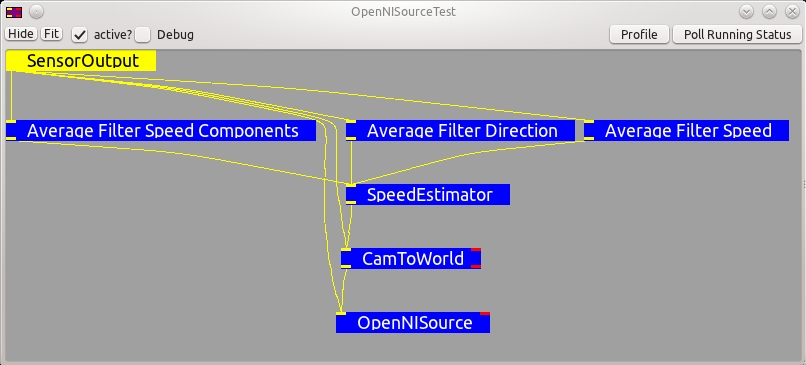
\includegraphics[scale=0.5]{graphics/OpenNISourceTest.jpg}
\caption{\label{fig:OpenNISourceTest} Die \lstinline{MCA2}-Grundstruktur
unseres Moduls in \lstinline{MCABrowser}}
\end{figure}

Zur Geschwindigkeitsschätzung wird der Torso (Rumpfmittelpunkt) auf den Boden projiziert
 (die Z-Koordinate – im Welt-Koordinatensystem - wird auf 0 gesetzt). Da die
 Positionsinformation wegen der hohen \gls{fps}-Rate mit viel Rauschen belastet wird
 (man bewegt sich langsam, die geringe Auflösung der Kinect aber interpretiert
 dies jedoch als geringfügige Posenänderungen im Ruhezustand.), muss die Positionveränderungen
 in größeren Zeitschritten ausgewertet werden. Dazu verwenden wir einen Glättungsfilter über
 je 5 Bilder (\lstinline{Average Filter Speed Components}, \lstinline{Average Filter Direction}, \lstinline{Average Filter Speed}).
 
Bevor die Geschwindigkeit für eine Abtastperiode aus der Differenz von den
aktuellen und vorherigen Werten kalkuliert wird (\lstinline{Speed Estimator}),
müssen die Koordinaten aus dem Kinect-Koordinatensystem in Roboterkoordinaten transformiert werden
 (\lstinline{CamToWorld}). Dieser Schritt benötigt die Kamerakalibration des
 Kinect-Sensors. Dies muss nur einmal gemacht werden, und kann mit \gls{opencv} oder
 in MATLAB (Camera Calibration Toolbox) durchgeführt werden. Die Ergebnisse (die extrinsischen Parameter)
 sollen durch ein ``Init-File'' (``calibration\_data.txt'' genannt) für das
 Programm zur Verfügung stehen.
 Anhand dieser Datei stellt die Anwendung die ``Kamera zu Roboter'' Transformationswerte automatisch ein.
 
Noch eine wichtige Bemerkung zur Geschwindigkeitsberechnung: da die \gls{fps}-Rate
 sich kontinuierlich ändert, muss stets der aktuelle \gls{fps}-Wert eingeholt werden.
 Dazu wird eine Zeitmessung zwischen zwei Abtastwerten eingeholt.

Die Zeit wird in Sekunden, die Entfernungen und Bewegungen werden in Millimeter gemessen.
 Die verwendeten Einheiten sind mm (Position, Positionsveränderung), mm/sec
 (Geschwindigkeit), frame/sec (Frame-Rate) und rad (Winkel).

Die Gestenerkennung wurde in einem zweiten Modul (\lstinline{GestureClassifier})
umgesetzt, das in Laufzeit aus \lstinline{OpenNISource} aufgerufen wird.

Gesten können sowohl von einzelnen Körperteilen, wie der Hand, als auch vom gesamten Körper ausgeführt werden. Es existieren unzählige Körperhaltungen, Bewegungen, Gesichtsausdrücke und Handgesten, die für die Kommunikation von Mensch und Maschine eingesetzt werden können.

\todo[inline]{Bild Hamsa Skeleton-Modell und Hand-Modell}

\subsubsection{Probleme}
\authorsection{\editorhamza}

Die gleichmäßige Farbgebung und geringe Texturierung der Menschlichen Hand machen eine Erkennung von inneren Kanten und somit die Segmentierung einzelner nicht ausgestreckter Finger schwierig. 
Die hohen Geschwindigkeiten für Translation (bis 5m/s) und Rotation ($300^\circ/s$) die für die globale Handbewegung erreicht werden können und die relativ niedrigen Kamerafrequenzen zwischen 30 und 60 Herz machen ein durchgehendes Tracking sehr schneller Bewegungen nahezu unmöglich.
Damit haben  wir für den  Körpergesten  entschieden, die sicherer und einfacher beim Test sind. 
In unserem Fall brauchen wir maximal 4 Gesten. Diese Gesten müssen durch Armen , die am meisten frei beweglich sind,gebildet sein.  Die einfachste Idee war, dass wir die Winkeln  zwischen Armengelenke messen. Wenn die Messwerten sich  innerhalb des Toleranz-bereichs befinden, wird die Geste erkannt, sonst  wird es als undefinierte Geste betrachtet . 



\subsection{Gestenerkennung}
\authorsection{Kinect-Gruppe}

Ursprünglich sollte eine beliebig erweiterbare Struktur zur Gestenerkennung verwendet werden.
 Diesem Ansatz liegt ein binärer Entscheidungsbaum zu Grunde, dem den einzelnen
 Output-Mög"-lich"-kei"-ten (den Blätter des Baums, also den eigentlichen
 Gesten) Identifikationsnummern zugeordnet werden.

Diese Struktur bietet programmierungstechnisch eine generische Lösung. Sie funktioniert anatomisch universal,
 also unabhängig von konkreten Körpermaßen der Person, durch die Verwendung relativer Merkmale.
 Dies sind zum Beispiel Winkel zwischen bestimmten Körperteilen.
 
Aufgrund der groben Auflösung und der stark verrauschten Messwerte der Kinect musste der ursprüngliche Plan verworfen werden.
 Somit wurde eine weniger generische, aber robuste Variante implementiert. Diese kann vier Basisbefehle deuten, die der Roboter zu seinem richtigen Betrieb benötigt.
\vspace{0.3cm}

\noindent Eingesetzte Geste und ihre Bedeutungen:
\begin{description}
  \item[Undefined gesture] (normal posture: any other cases except the ones
  listed below)
  \item[Start follow me] 
  $[if: (angle\_alpha > 45^\circ$ $\&\&$ $angle\_beta >
  45^\circ)$\\
  $\&\&$ $(angle\_gamma > 135^\circ$ $\&\&$ $angle\_delta >
  135^\circ)$\\
  $\&\&$ $((left\_hand\_z - right\_hand\_z) > 300 mm)]$
  \item[Stop follow me] $[if: (angle\_alpha > 45^\circ$ $\&\&$ $angle\_beta >
  45^\circ)$\\
  $\&\&$ $(angle\_gamma > 135^\circ$ $\&\&$ $angle\_delta > 135^\circ)$\\
  $\&\&$ $((right\_hand\_z - left\_hand\_z) > 300 mm)]$
  \item[Stop] $[if: (angle\_alpha > 45^\circ$ $\&\&$ $angle\_beta > 45^\circ)$\\
  $\&\&$ $(angle\_gamma > 135^\circ \&\& angle\_delta > 135^\circ)$\\
  $\&\&$ $(|right\_hand\_z - left\_hand\_z| < 300 mm)]$
  \item[Repeat track] $[if: (angle\_alpha > 45^\circ$ $\&\&$ $angle\_beta >
  45^\circ)$\\
  $\&\&$ $(angle\_gamma < 135^\circ || angle\_delta < 135^\circ)]$
\end{description}

\begin{table}[h]
\centering
\begin{tabular}{ll}
\textbf{Undefined gesture} & (normal posture: any other cases except the ones
 listed below)\\
 &\\
 &\\
\textbf{Start follow me} & $[if: (angle\_alpha > 45^\circ$ $\&\&$ $angle\_beta >
  45^\circ)$ $\&\&$\\
  & $(angle\_gamma > 135^\circ$ $\&\&$ $angle\_delta >
  135^\circ)$ $\&\&$\\
  & $((left\_hand\_z - right\_hand\_z) > 300 mm)]$\\
  &\\
  &\\
\textbf{Stop follow me} & $[if: (angle\_alpha > 45^\circ$ $\&\&$ $angle\_beta >
  45^\circ)$ $\&\&$\\
  & $(angle\_gamma > 135^\circ$ $\&\&$ $angle\_delta > 135^\circ)$ $\&\&$\\
  & $((right\_hand\_z - left\_hand\_z) > 300 mm)]$\\
  &\\
  &\\
\textbf{Stop} & $[if: (angle\_alpha > 45^\circ$ $\&\&$ $angle\_beta >
45^\circ)$ $\&\&$\\
 & $(angle\_gamma > 135^\circ \&\& angle\_delta > 135^\circ)$ $\&\&$\\
 & $(|right\_hand\_z - left\_hand\_z| < 300 mm)]$\\
 &\\
 &\\
\textbf{Repeat track} & $[if: (angle\_alpha > 45^\circ$ $\&\&$ $angle\_beta >
  45^\circ)$ $\&\&$\\
 & $(angle\_gamma < 135^\circ || angle\_delta < 135^\circ)]$
\end{tabular}
\caption{Eingesetzte Geste und ihre Bedeutungen}
\label{tab:Gesten}
\end{table}

\todo[inline]{Auswählen ob Tabelle oder Description verwendet werden soll}

\begin{figure}[h]
\center
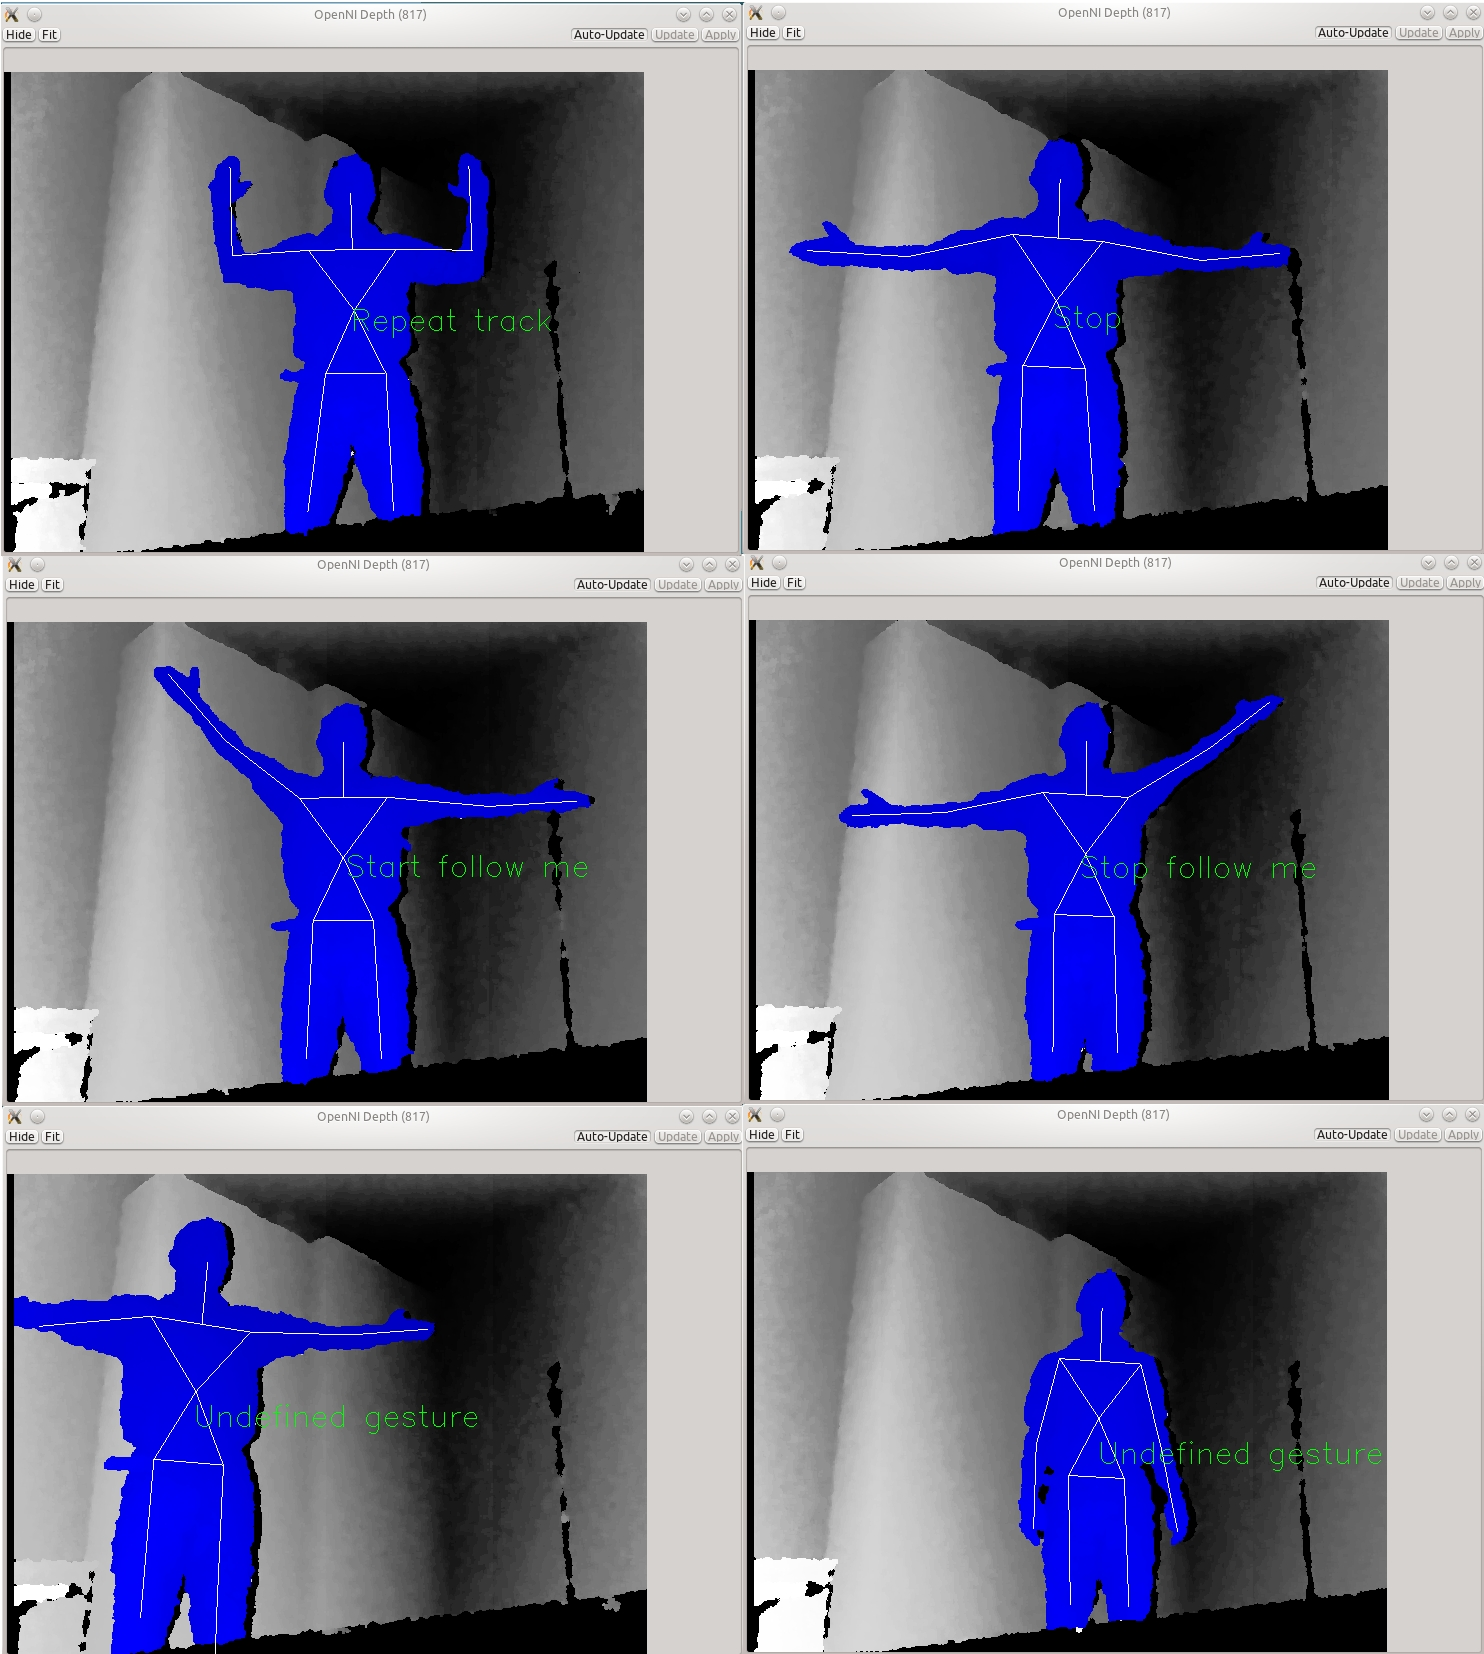
\includegraphics[scale=0.25]{graphics/Gesten.jpg}
\caption[Definierte Gesten]{\label{fig:Gesten} Die vier definierten Gesten (oben und in der Mitte),
 bzw. die beiden Möglichkeiten für unbestimmte Fälle (links unten: mangelndes Gelenk, rechts unten: normale Körperhaltung)}
\end{figure}

\begin{table}[h]
\centering
\begin{tabular}{ll}
angle\_alpha: & angle between elbow $\rightarrow$ shoulder $\rightarrow$ hip on
the left side\\
angle\_beta: & angle between elbow $\rightarrow$ shoulder $\rightarrow$ hip on
the right side\\
angle\_gamma: & angle between shoulder $\rightarrow$ elbow $\rightarrow$ hand on
the left side\\
angle\_delta: & angle between shoulder $\rightarrow$ elbow $\rightarrow$ hand on
the right side\\
angle\_epsilon: & angle between neck $\rightarrow$ shoulder $\rightarrow$ elbow
on the left side\\
angle\_fi: & angle between neck $\rightarrow$ shoulder $\rightarrow$ elbow on
the right side\\
left\_hand\_z: & height of left hand (palm)\\
right\_hand\_z: & height of right hand (palm)\\
\end{tabular}
\caption{Erklärung zu charakteristischen Markmalen (Winkeldefintionen)}
\label{tab:Winkeldefintionen}
\end{table}

Falls eines der relevanten Gelenke verdeckt ist oder keine verfolgbare Person im
Sichtbereich der Kamera ist, wird automatisch \lstinline{UNDEFIED_GESTURE}
zurückgegeben. Dies ist eine vorbeugende Maßnahme gegen falsche Berechnungen.

Eine weitere Möglichkeit der Umsetzung ist das Erkennen des zeitlichen Verlaufs von Gesten (bspw. Winken, Kreisen).
 In \gls{openni} und NITE Modulen wurden solche Funktionen implementiert, jedoch konnten wir diese aufgrund von Konfigurationsproblemen nicht nutzen.
Bei der Anwendung werden stets einzelne Personen verfolgt. Sollten sich mehrere Personen im Sichtfeld der Kamera aufhalten, wird nur die zuerst getrackte Person beachtet.

\subsection{Fazit}
Im Mobile Roboter -- Praktikum hatten wir die Gelegenheit aktuelle
 Forschungsgebiete der Servicerobotik zu beleuchten und verschiedene
 Technologien praktisch auszuprobieren. Es fiel besonders auf, dass viele Konzepte zwar theoretisch funktionieren,
 jedoch in der der Praxis nicht umsetzbar waren. Dies bedingte einige Iterationen im ursprünglichen Zielsystem des Projekts
 wodurch der Funktionsumfang der letztendlichen Roboterplattform weitaus geringer ausfiel als geplant.
 Besonders in der Bildverarbeitung gab es erhebliche Probleme, da Softwarebibliotheken eingesetzt werden sollten,
 die sich selbst noch stark in der Entwicklung befanden. Somit konnte zum Beispiel die in NITE implementierte Gestenerkennung
 nicht verwendet werden und die Sensordaten der Kinect waren weitaus stärker verrauscht als erwartet.
 
Die Aufteilung der Gruppe in drei spezialisierte Teilgruppen war bei dem Umfang des Projekts sehr sinnvoll,
 das Projektmanagement jedoch schlecht. In den Teams wurde es versäumt früh feste Strukturen und Arbeitsweisen zu implementieren wodurch
 wenig zielorientiertes Arbeiten und großer Motivationsschwund entstanden. Letztendlich konnte das Ziel des Projekts jedoch erreicht werden.
